\chapter{Program Documentation}
\label{chap:program}

This chapter focuses on the implementation part of the thesis.

\section{Overview}
As mentioned, suggestions are retrieved by a REST API call made to the Web module. This module processes the data and
invokes the Suggester module to return the suggestions. Simplified diagram which show the main interactions between the
objects and modules can be seen in the figure \ref{programmer_sequence}.
\begin{figure}[htbp]
    \centering
    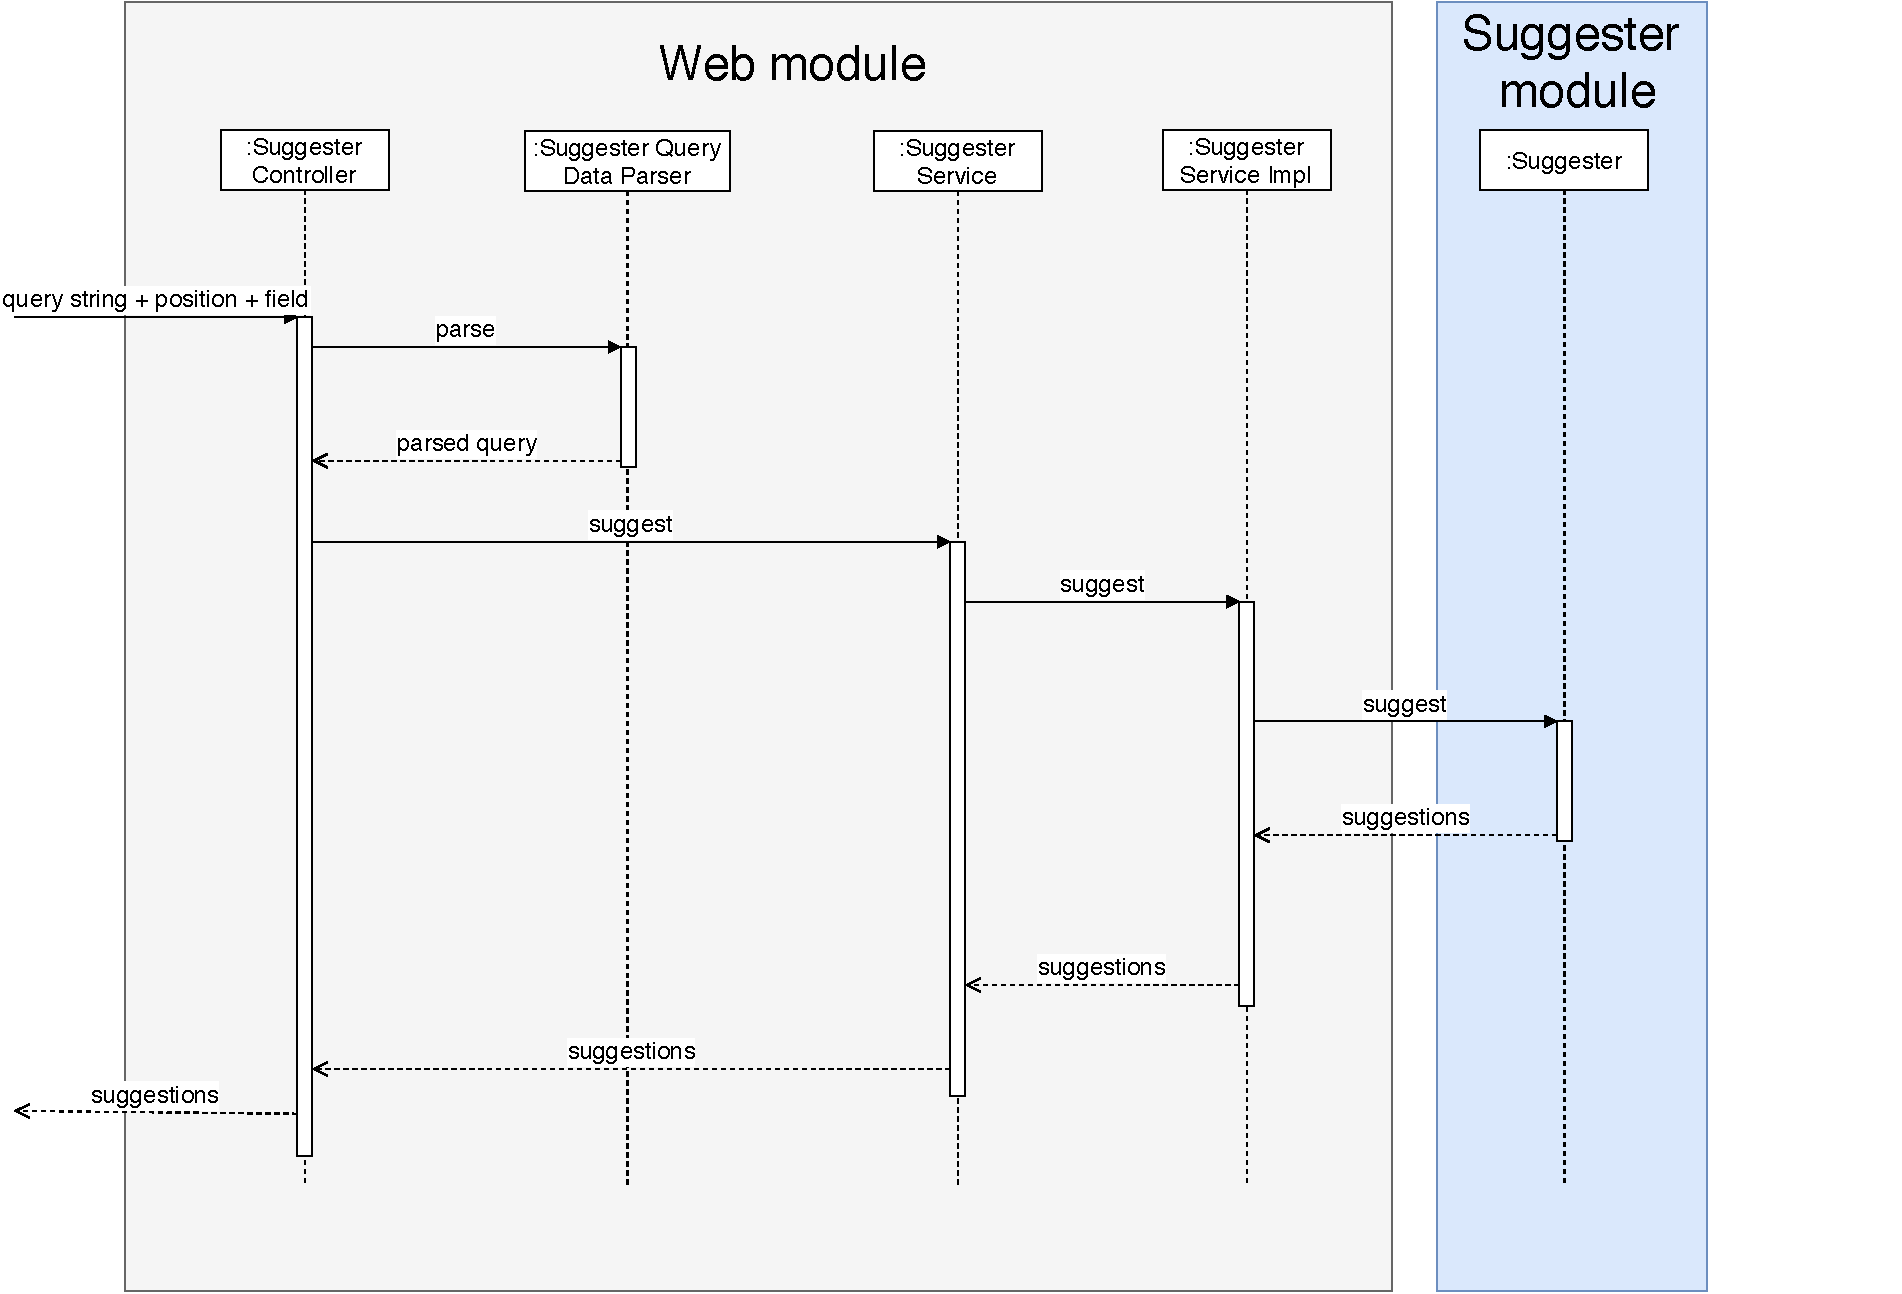
\includegraphics[width=145mm]{../img/programmer_sequence.pdf}
    \caption{Overview of the main object interactions}
    \label{programmer_sequence}
\end{figure}

\section{Web module}

\section{Suggester module}

\subsubsection{Public API}

\subsubsection{Suggester data}

\subsubsection{Detecting index version}

\subsubsection{Configuration change}

\subsubsection{Data structures abstractions}

\section{Testing}
Unit tests\footnote{\url{https://en.wikipedia.org/wiki/Unit_testing}} were written for the Suggester module to test
the basic functionality. They can be found in a standard Maven test directory \textit{src/test/java}.

To test the real word usage and to test the integration with other OpenGrok modules,
tests were written for \textit{SuggesterController} which test the
suggester endpoint in the Web module which in turn calls various parts from Indexer and Suggester modules.
Small projects written in variety of programming languages used for OpenGrok's own testing were used as test data.
These can be found in \textit{testdata/sources} directory of the OpenGrok project root.
First of all, these projects are copied into the temporary \textit{sourceRoot} directory. Then they are indexed.
After that, the Suggester is initialized. Finally, the tests run.

However, the tests are not exhaustive and for better test coverage more tests should be written.

As for UI testing, OpenGrok does not have any UI tests in place. Therefore, it was not deemed to be a high priority.
In the future, it would make sense to incorporate at least some UI testing.